\documentclass[journal]{IEEEtranTIE}

\usepackage{graphicx}
\usepackage{cite}
\usepackage{picinpar}
\usepackage{amsmath}
\usepackage{amssymb}
\usepackage{url}
\usepackage{flushend}
\usepackage[utf8]{inputenc}
\usepackage{colortbl}
\usepackage{soul}
\usepackage{multirow}
\usepackage{pifont}
\usepackage{color}
\usepackage{alltt}
\usepackage[hidelinks]{hyperref}
\usepackage{enumerate}
\usepackage{subcaption}
\usepackage{siunitx}
\usepackage{breakurl}
\usepackage{epstopdf}
\usepackage{pbox}
\usepackage{booktabs}

\begin{document}

\title{W2Switch: Adaptive Reinforcement Learning Control for Industrial Filling}
% \title{SPARC-FILL: Switch-Point Adaptive Reinforcement Control for Industrial Filling}


\author{%
\"{O}mer Sabri Emeksiz,\ Engin Ma\c{s}azade, \emph{Member, IEEE},
and Suat Selim%
\thanks{Manuscript prepared Month~xx,~2024; revised Month~xx,~2024.}
\thanks{\"{O}.~S. Emeksiz is with Ko\c{c} University, Department of Computer Engineering, Istanbul 34450, Turkey (e-mail: oemeksiz24@ku.edu.tr).}
\thanks{E. Ma\c{s}azade is with Marmara University, Department of Electrical and Electronics Engineering, Istanbul 34722, Turkey (e-mail: engin.masazade@marmara.edu.tr).}
\thanks{S. Selim is with BAYKON Industrial Weighing Systems, Istanbul 34775, Turkey (e-mail: sselim@baykon.com).}}

\maketitle

\begin{abstract}
This placeholder abstract will later capture the motivation, reinforcement learning strategy, and major findings from the filling control study.
\end{abstract}

\begin{IEEEkeywords}
Reinforcement learning, industrial automation, filling control, multi-armed bandits, Monte Carlo methods
\end{IEEEkeywords}

\markboth{IEEE Transactions on Industrial Electronics}{}

\section{Industrial Motivation and Application Overview}
\begin{itemize}
  \item Lay out the production challenges that trigger the need for automated switch-point decisions.
  \item Emphasize safety, quality, and throughput goals that motivate the reinforcement learning approach.
  \item Introduce the industrial partner and anticipated operational impact.
\end{itemize}

\section{Filling Device and Instrumentation}
\begin{itemize}
  \item Summarize the filling machine hardware, two-stage actuator design, and sensing capabilities.
  \item Explain how switch timing influences valve behavior, product quality, and cycle time.
  \item Document control interfaces, communication protocols, and any hardware constraints.
\end{itemize}

\section{Process Data Acquisition and Characterization}
The filling device described in Section~II was loaded with iron particles and operated in production mode while the target weight was fixed at \SI{750}{\gram} with a $\pm\SI{10}{\gram}$ tolerance. For each experiment we selected a candidate switch point, triggered the coarse-to-fine valve transition, and logged the hopper weight every \SI{10}{\milli\second}. The embedded controller exposes these samples through its TCP interface: the microcontroller streams a semicolon-separated list of instantaneous weights, augmented with two flags that mark (i) the instant the valve mode changes and (ii) the moment the motor stops. Because residual material continues to fall after the stop command, the payload also includes the stabilised termination weight that defines the delivered mass.

We captured 1\,108 fillings under these conditions. The safe operating region is defined as $\SI{740}{\gram} \le \bar{w} \le \SI{760}{\gram}$, and the dataset contains examples both inside and outside this band. Descriptive statistics are summarised in Table~\ref{tab:data-stats}, while Fig.~\ref{fig:data-hist} and Fig.~\ref{fig:data-avglen} illustrate the weight sample distribution and the spread of episode lengths recorded in the historian.

Before clustering, the raw TCP streams are parsed, the coarse/fine and stop markers are converted into explicit indices, and corrupted runs are filtered out. The first \SI{500}{\milli\second} of each trace are discarded to account for valve opening lag and sensor stabilisation, which otherwise yield negative or unreliable readings. Weight samples are then converted from the decigram counts emitted by the device to grams and quantised in \SI{10}{\gram} steps to match the firmware resolution. Episodes lacking either marker or exhibiting excessive noise are removed. The remaining traces are archived in the historian as one column per filling, which are subsequently loaded into the clustering procedure. The resulting coverage across switch points is illustrated in Fig.~\ref{fig:session-counts} and underpins the training curriculum described next.

\begin{table}[t]
  \centering
  \caption{Summary statistics of the collected filling dataset ($N=1{,}108$).}
  \label{tab:data-stats}
  \begin{tabular}{l c}
    \toprule
    Metric & Value \\
    \midrule
    Total fillings & $1\,108$ \\
    Average fill time & $3.26 \pm 0.97$~s \\
    Median fill time & $2.95$~s \\
    $90^{\mathrm{th}}$ percentile fill time & $4.70$~s \\
    Average switch point & \SI{543.2}{\gram} \\
    Average final weight & \SI{767.6}{\gram} \\
    Safe fillings & $772$ \\
    Overflow count & $303$ \\
    Underflow count & $33$ \\
    \bottomrule
  \end{tabular}
\end{table}

\begin{figure*}[t]
  \centering
  \begin{subfigure}{0.32\textwidth}
    \centering
    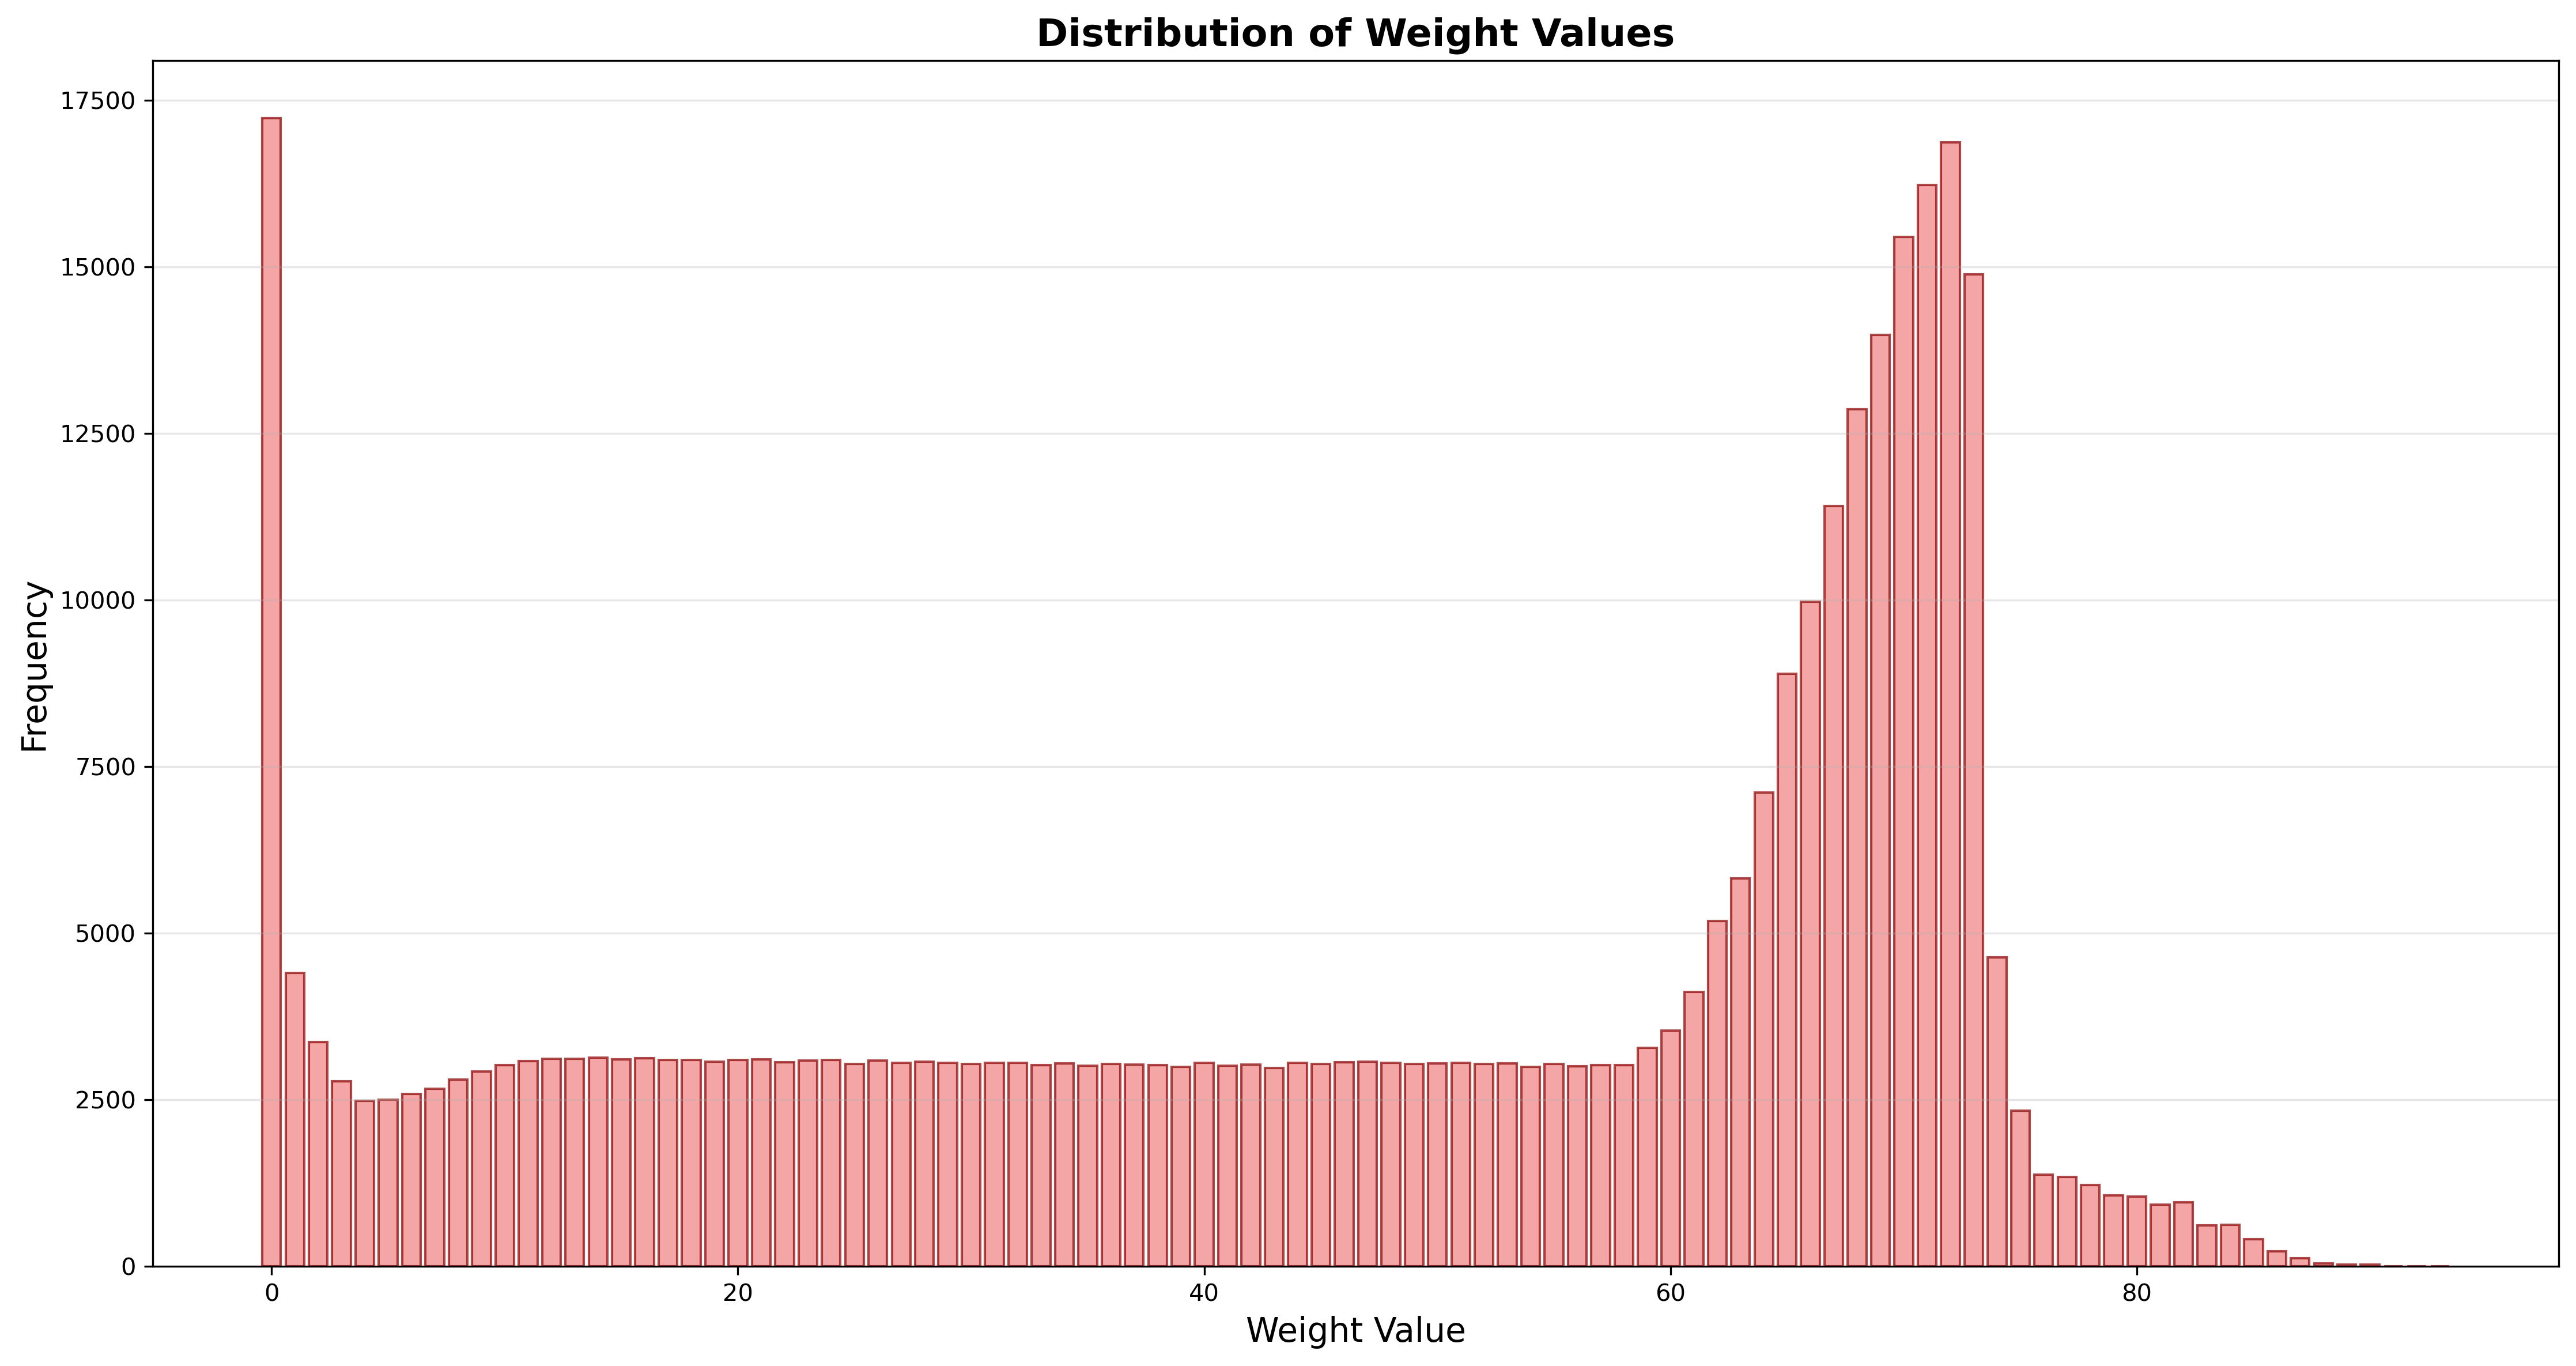
\includegraphics[width=\linewidth]{figures/weight_count_histogram.png}
    \caption{Weight sample distribution.}
    \label{fig:data-hist}
  \end{subfigure}
  \hfill
  \begin{subfigure}{0.32\textwidth}
    \centering
    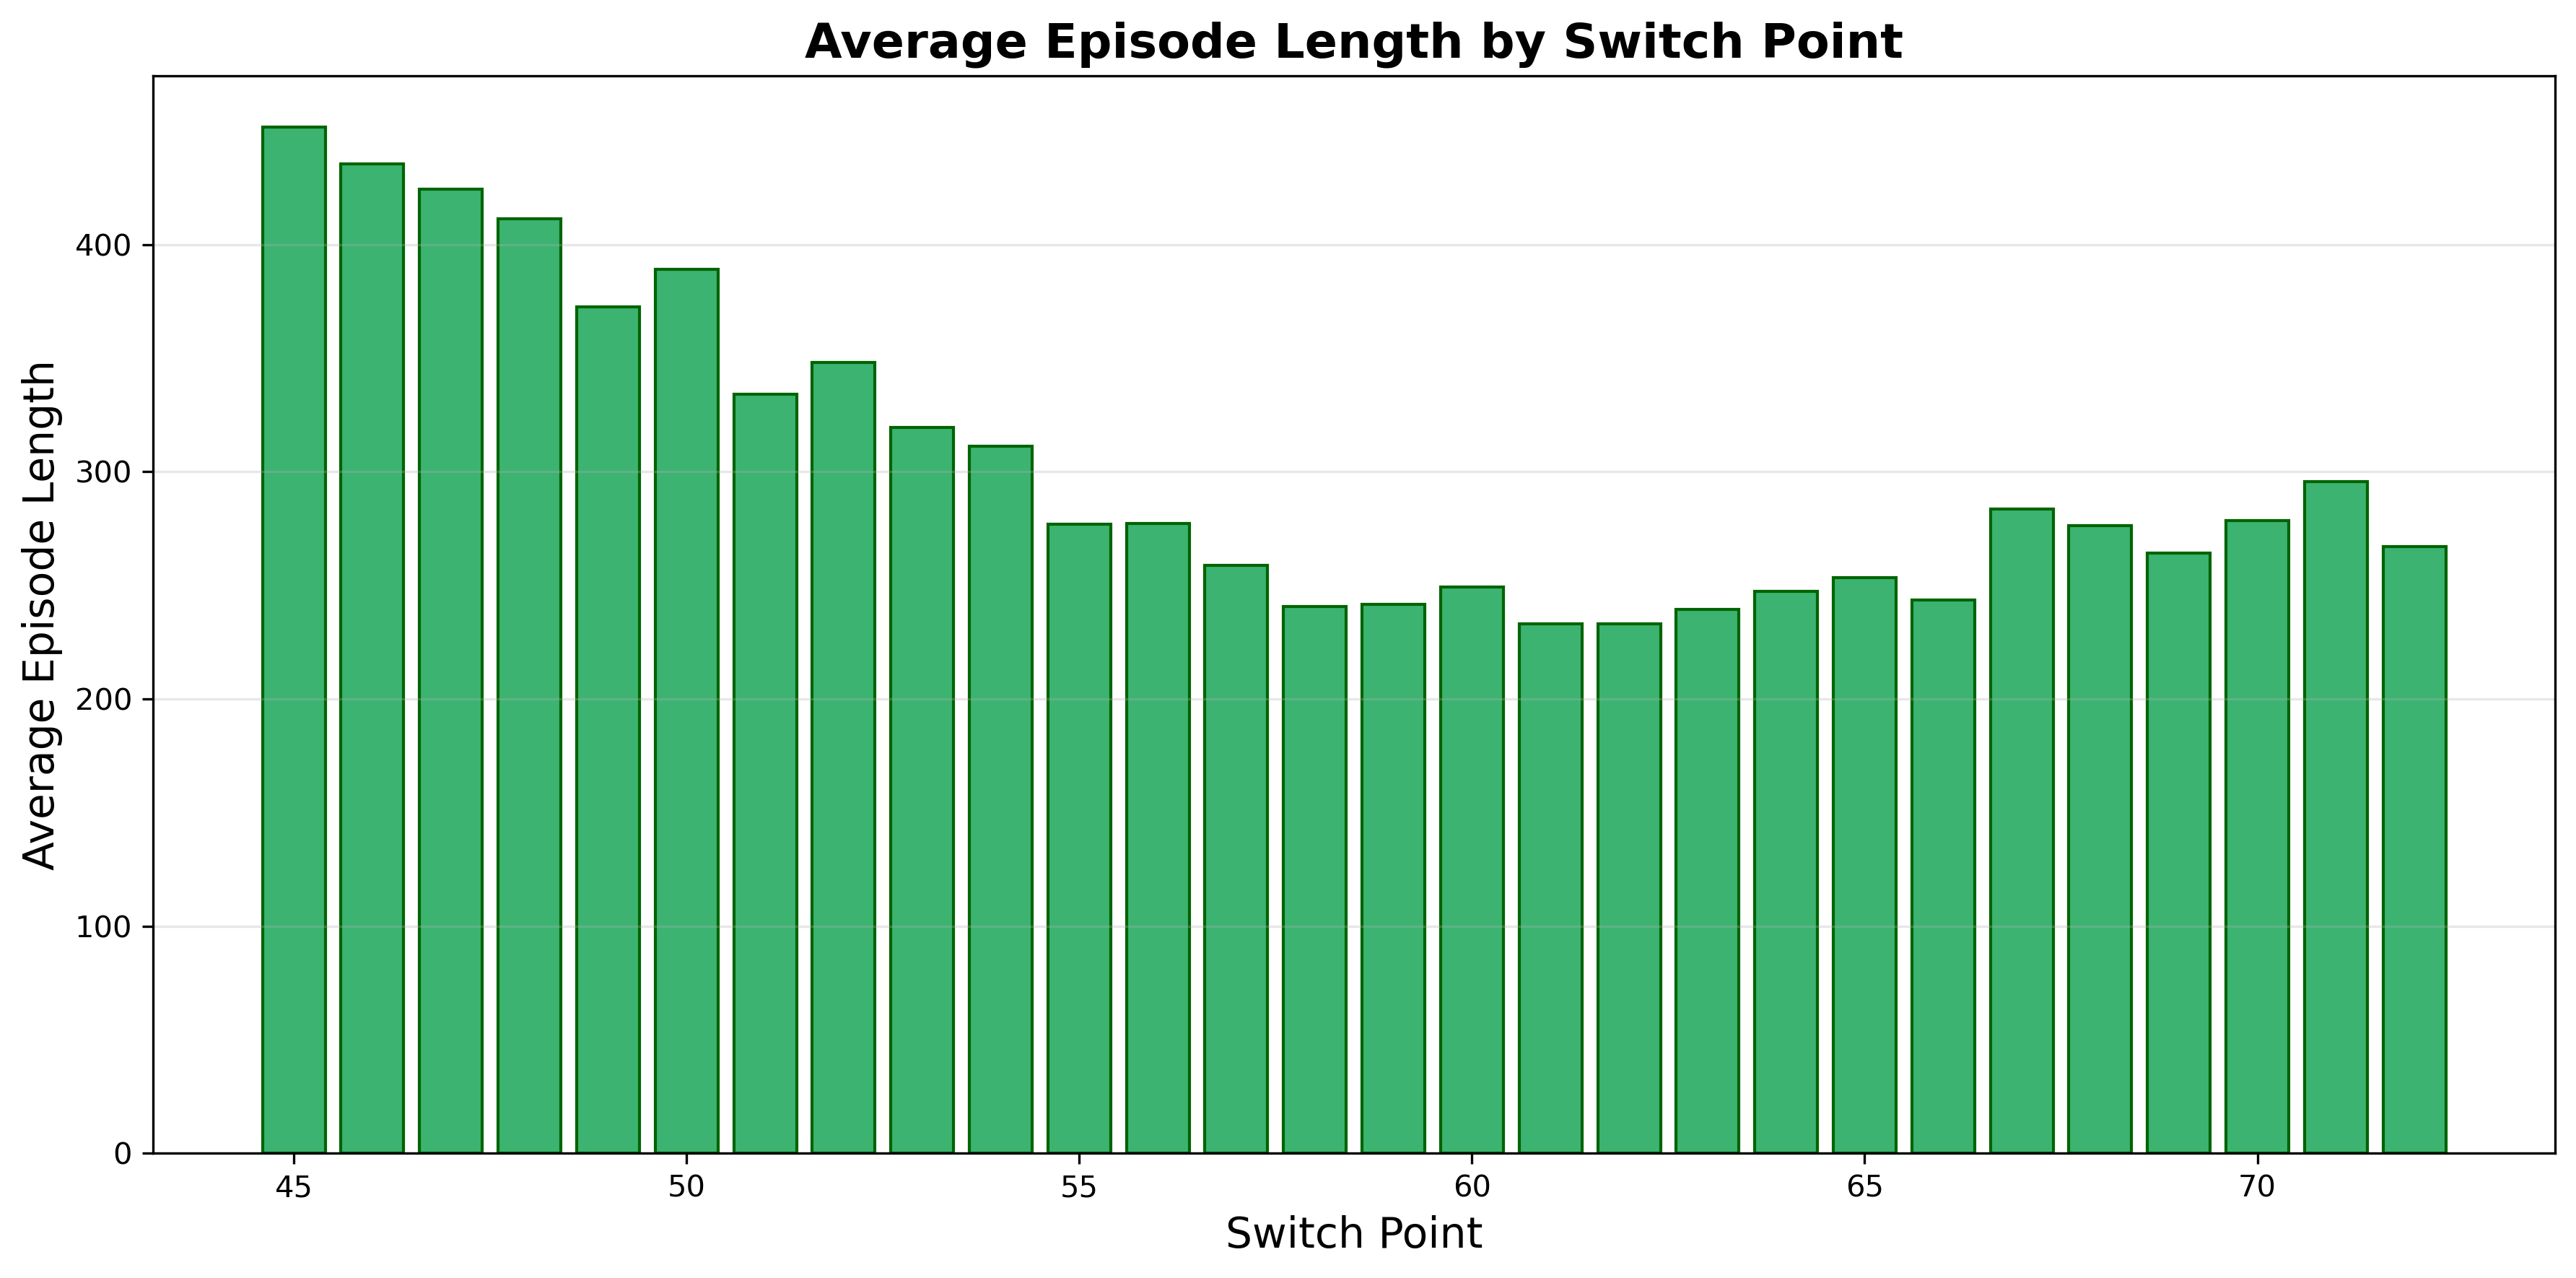
\includegraphics[width=\linewidth]{figures/avg_episode_length_by_switch.png}
    \caption{Average episode length per switch.}
    \label{fig:data-avglen}
  \end{subfigure}
  \hfill
  \begin{subfigure}{0.32\textwidth}
    \centering
    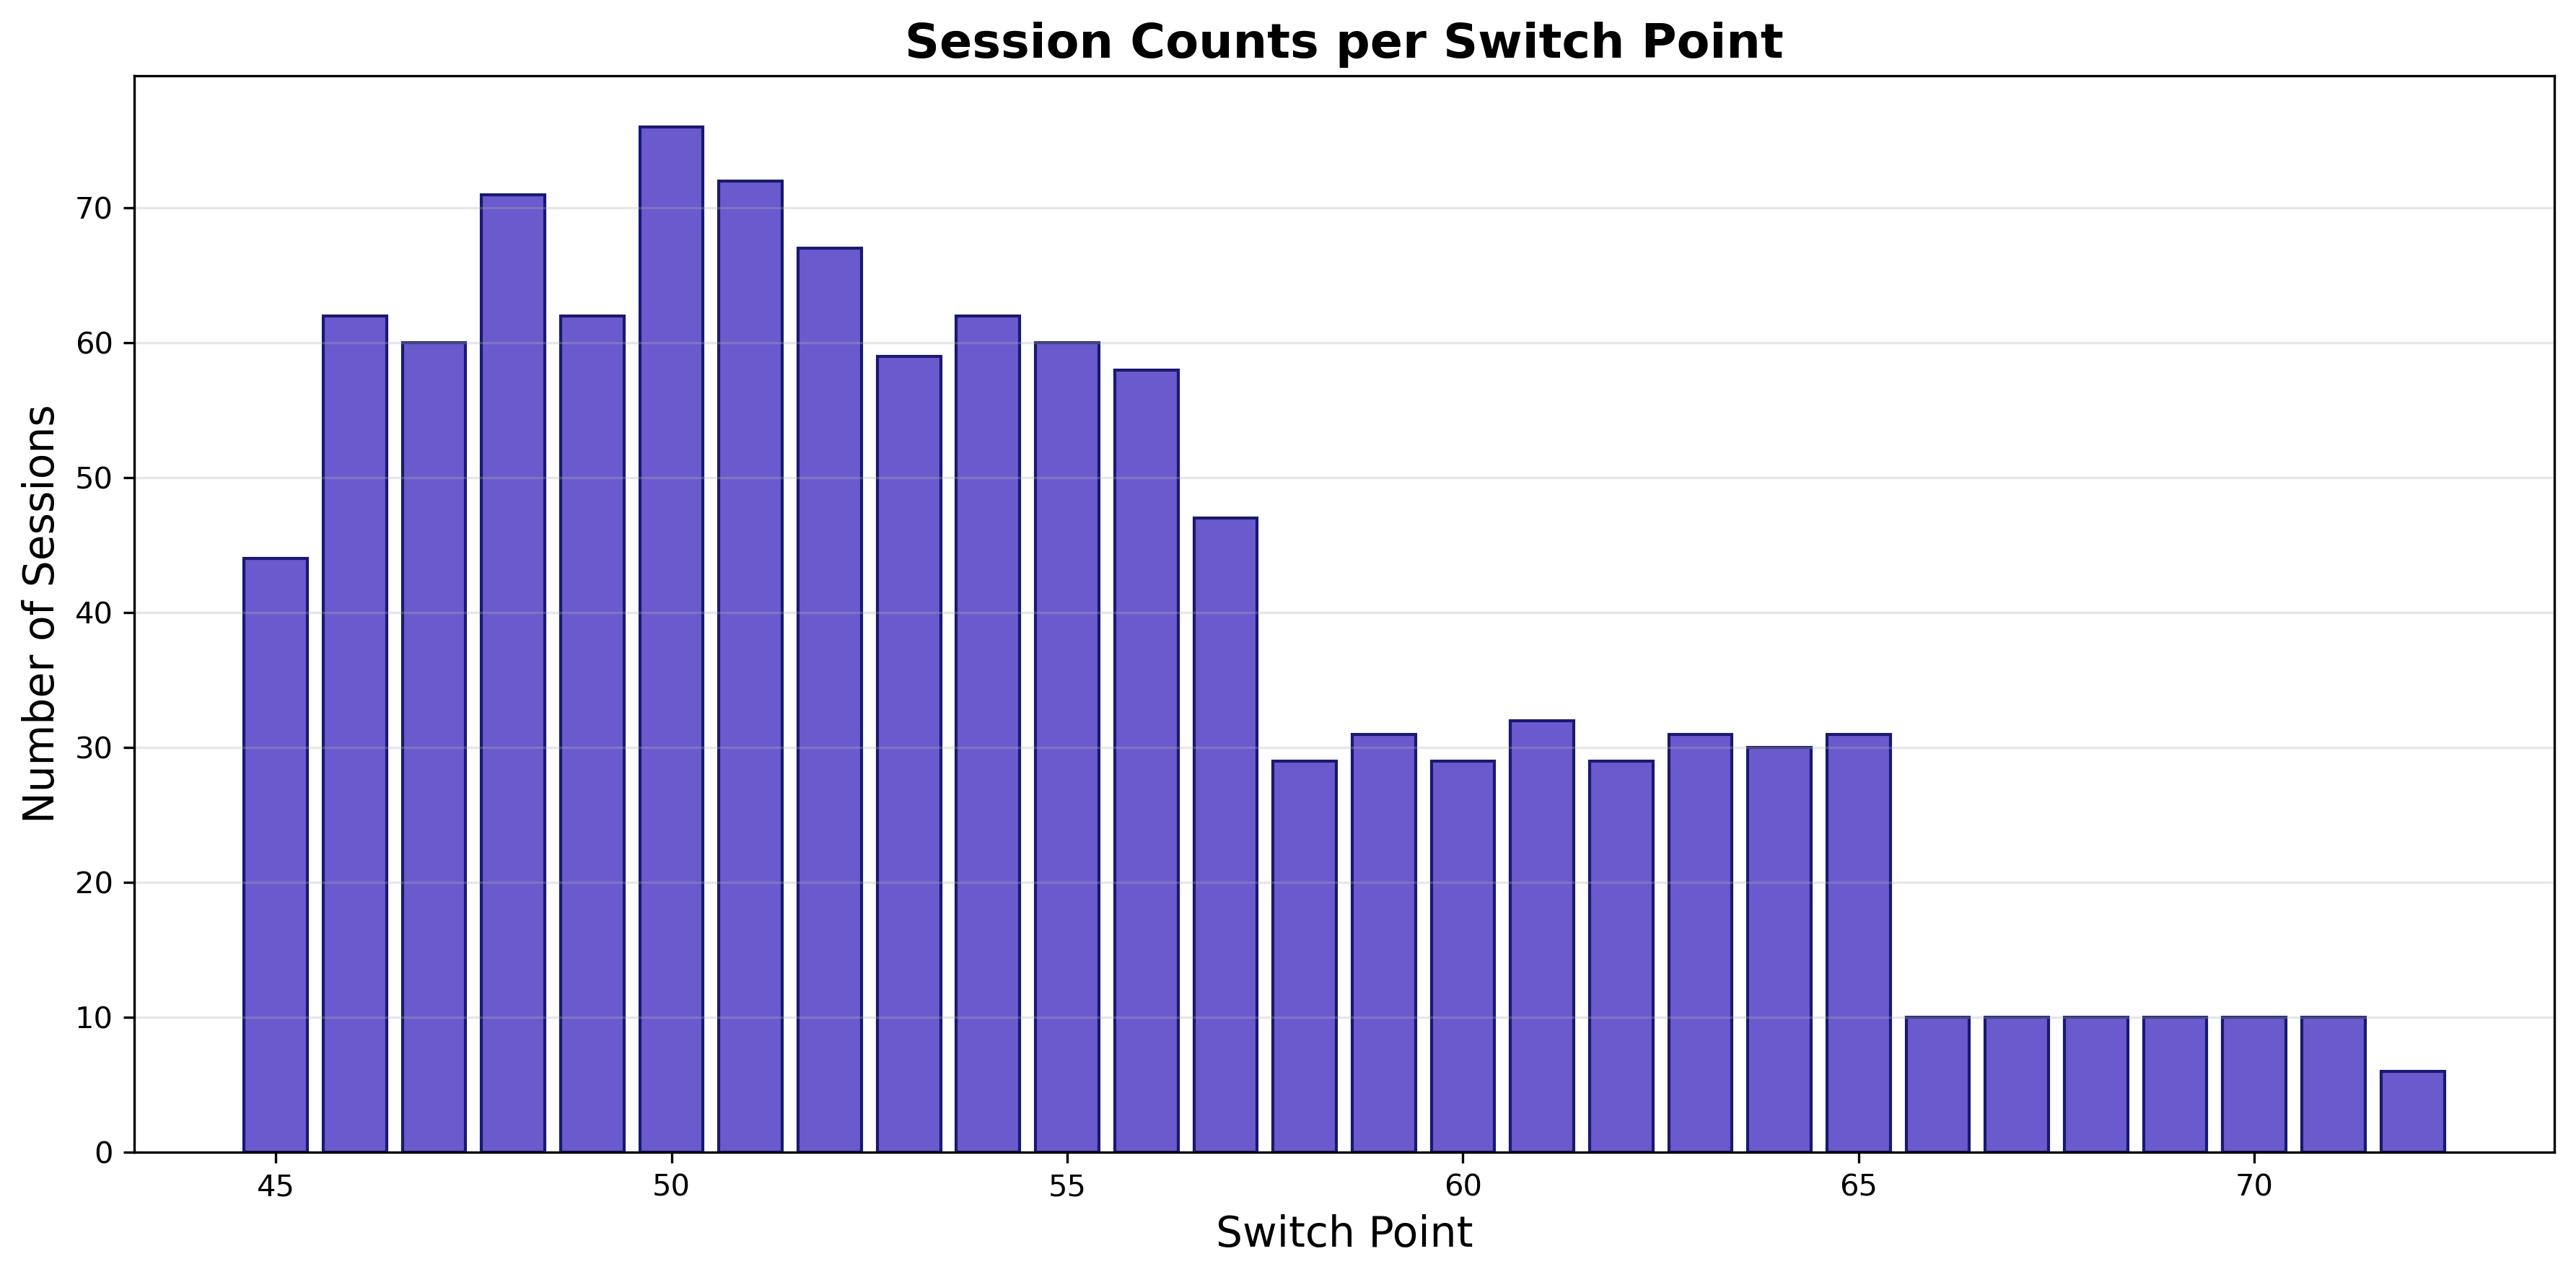
\includegraphics[width=\linewidth]{figures/session_counts_by_switch.png}
    \caption{Sessions available per switch.}
    \label{fig:session-counts}
  \end{subfigure}
  \caption{Data characterisation plots derived from the historian logs.}
  \label{fig:data-overview}
\end{figure*}

\section{Switch Point Clustering and Training Setup}
Operator logs provide an explicit time stamp for the fast-to-slow transition that closed each historical cycle. We use this marker to cluster the dataset into disjoint episode sets $\{\mathcal{E}(s)\}_{s\in\mathcal{S}}$, where every member of $\mathcal{E}(s)$ was executed with the same switching point $s$. This simple partitioning exposes the empirical variability around each candidate switch while preserving the causal ordering of events recorded on the line. Before training starts we verify that every cluster contains at least one usable trajectory and trim the candidate list $\mathcal{S}$ to the intersection of switch points observed consistently across operators. This guardrail prevents the controller from proposing thresholds that never appear in practice.

Training mirrors the way the embedded device will operate. Each learning episode begins by selecting a switch candidate (either the initial seed or the value returned by the previous decision step), drawing one unused trajectory from the corresponding cluster, and feeding the observed length $L_t$ and final weight $\bar{w}_t$ back to the agent. After the sample is consumed we mark it as unavailable so that repeated visits to the same switch point encounter different realizations, just as the real plant would. The available data cover every candidate switch with several trajectories (Fig.~\ref{fig:session-counts}), ensuring that each cluster can support multiple visits before the round-robin reset is needed. This sequential sampling contrasts with the naive alternative of shuffling the entire dataset: random playback would expose the agent to the consequences of many different switch points without ever requiring it to decide when the transition should occur, leading to misleading value estimates and slow or unstable convergence. By forcing the loop “pick switch $\rightarrow$ observe filling outcome $\rightarrow$ update policy,” we ensure that offline training faces the same credit-assignment structure as the online deployment.

When the exploration policy proposes a switch that exhausts its cluster, the sampler wraps around and starts reusing trajectories only after all available switch points have been visited once. This round-robin schedule maintains a balanced curriculum, avoids overfitting to a handful of favourable traces, and keeps the distribution of training episodes aligned with the distribution encountered during testing. Combined with the guardrails on $\mathcal{S}$, the clustering-based setup therefore delivers a faithful stand-in for the production environment while remaining fully reproducible in the offline toolbox.

\begin{figure*}[t]
  \centering
  \includegraphics[width=0.9\textwidth]{figures/rlfc_diagram.png}
  \caption{Overview of the proposed workflow. Offline logs flowing from the historian are clustered by switch point so the agent samples episodes exactly as they will appear on the device. The resulting policy drives the device-in-the-loop validation loop, where fresh fillings are logged back to the database for replay and monitoring.}
  \label{fig:pipeline}
\end{figure*}

\section{Reinforcement Learning Framework}
\label{sec:rl-framework}
Offline production logs are transformed into episodes $\{w_k\}_{k=0}^{T_e}$ with annotated switch points $s^{\text{op}}_e$, cycle durations $L_e$, and realised masses $\bar{w}_e$. For every candidate $s\in\mathcal{S}=\{s_1,\dots,s_{|\mathcal{S}|}\}$ we denote by $\mathcal{E}(s)$ the set of episodes associated with that switch point. The agents access the same discretised weight bins $\mathcal{W}$ and action set $\mathcal{A}=\{+1,-1\}$ (coarse and fine feed).

\subsection{State, Action, and Reward Design}
Both learning agents share the same penalty function
\begin{equation}
  \mathcal{P}(\bar{w}) =
  \begin{cases}
    -C_{\mathrm{ov}}\,(\bar{w}-w_{\max}), & \bar{w}>w_{\max},\\[2pt]
    -C_{\mathrm{un}}\,(w_{\min}-\bar{w}), & \bar{w}<w_{\min},\\[2pt]
    0, & \text{otherwise},
  \end{cases}
  \label{eq:penalty}
\end{equation}
where $C_{\mathrm{ov}}$ and $C_{\mathrm{un}}$ denote the overflow and underflow penalties, respectively, and $[w_{\min},w_{\max}]$ is the contractual tolerance window. The multi-armed bandit (MAB) consumes each episode as a single reward signal
\begin{equation}
  r^{\mathrm{mab}}(L,\bar{w}) = -L + \mathcal{P}(\bar{w}),
  \label{eq:mab_reward}
\end{equation}
so the cycle-time penalty is injected explicitly through the episode length $L$, while $\mathcal{P}(\bar{w})$ captures final-weight deviations. The Monte Carlo (MC) agent instead spreads the cycle-time penalty over intermediate transitions by assigning the per-sample cost $c=-1$ before the switch point and reserving the terminal penalty for quality deviations:
\begin{equation}
  r_k =
  \begin{cases}
    c, & 0 \le k < T_e-1,\\[2pt]
    c + \mathcal{P}(\bar{w}_e), & k = T_e-1.
  \end{cases}
  \label{eq:step_reward}
\end{equation}
Exploration for both agents follows an $\epsilon$-greedy policy that is biased toward forward neighbours in $\mathcal{S}$. With exploration probability $\epsilon_t$ at episode $t$ and decay factor $\lambda\in(0,1)$, the schedule evolves according to
\begin{equation}
  \epsilon_{t+1} = \max\bigl(\epsilon_{\min},\,\lambda\,\epsilon_t\bigr),
  \label{eq:epsilon_schedule}
\end{equation}
and roulette-wheel sampling over a user-defined set of step weights determines the offset $\Delta s\in\{0,+1,+2,\dots\}$ applied to the current best switch point. When exploration is inactive ($\Delta s=0$) the agent repeats the incumbent optimum to avoid abrupt changes on the plant; we denote this sampling routine by \textsc{SelectSwitch}$(s,Q,\epsilon)$ when it receives the reference switch and the current value estimates.

\subsection{Multi-Armed Bandit Controller}
The multi-armed bandit (MAB) treats every candidate $s\in\mathcal{S}$ as an arm with value $Q(s)$. During episode $t$ the agent executes $s_t$, retrieves an unused trajectory from $\mathcal{E}(s_t)$, and evaluates the scalar reward $r_t=r^{\mathrm{mab}}(L_t,\bar{w}_t)$ from~\eqref{eq:mab_reward}. Action values follow a running-average update (summarised in Fig.~\ref{fig:mab-pseudocode})
\begin{equation}
  Q_{t+1}(s_t) = Q_t(s_t) + \frac{1}{N_t(s_t)+1}\bigl(r_t - Q_t(s_t)\bigr),
  \label{eq:mab_update}
\end{equation}
where $N_t(s)$ counts how many times arm $s$ has been visited prior to episode $t$. Using the visit count instead of a fixed stepsize avoids over-weighting early samples when the availability of $\mathcal{E}(s)$ differs across switch points, which would otherwise bias the arm estimates. Exploitation picks $s^\star_t = \arg\max_{s\in\mathcal{S}} Q_t(s)$, while exploration samples $s_{t+1}$ by applying the offset drawn via~\eqref{eq:epsilon_schedule} to $s^\star_t$. Because the data processor marks trajectories as consumed, subsequent updates associated with the same $s$ reflect different production runs, allowing the bandit to build statistics about variability in overfill and underfill outcomes. At convergence the recommended operating point is $s^\star = \arg\max_s Q_T(s)$, and the training logs capture both the learning curve and the evolution of empirical visitation counts.

\begin{figure}[t]
  \centering
  \begingroup\footnotesize
  \begin{tabular}{p{0.95\linewidth}}
    \toprule
    \textbf{Inputs:} $\mathcal{S}$, $\{\mathcal{E}(s)\}_{s\in\mathcal{S}}$, $T$, $(\epsilon_0,\epsilon_{\min},\lambda)$, $s_{\mathrm{curr}}$ \\
    \textbf{Outputs:} $Q^{\mathrm{mab}}(s)$, $s^\star$ \\
    \midrule
    Initialise $Q^{\mathrm{mab}}(s)\leftarrow 0$, $N^{\mathrm{mab}}(s)\leftarrow 0$; set $\epsilon\leftarrow\epsilon_0$ \\
    \textbf{for} $t=1$ \textbf{to} $T$ \textbf{do} \\
    \quad $s_t \leftarrow \textsc{SelectSwitch}(s_{\mathrm{curr}}, Q^{\mathrm{mab}}, \epsilon)$ \\
    \quad Sample $\sigma_t \in \mathcal{E}(s_t)$; extract $L_t$, $\bar{w}_t$ \\
    \quad $r_t^{\mathrm{mab}} \leftarrow -L_t + \mathcal{P}(\bar{w}_t)$ \\
    \quad $N^{\mathrm{mab}}(s_t) \leftarrow N^{\mathrm{mab}}(s_t)+1$ \\
    \quad $Q^{\mathrm{mab}}(s_t) \leftarrow Q^{\mathrm{mab}}(s_t) + \dfrac{r_t^{\mathrm{mab}} - Q^{\mathrm{mab}}(s_t)}{N^{\mathrm{mab}}(s_t)}$ \\
    \quad $\epsilon \leftarrow \max(\epsilon_{\min}, \lambda \epsilon)$; $s_{\mathrm{curr}} \leftarrow s_t$ \\
    \textbf{end for} \\
    $s^\star \leftarrow \arg\max_{s\in\mathcal{S}} Q^{\mathrm{mab}}(s)$ \\
    \bottomrule
  \end{tabular}
  \endgroup
  \caption{Pseudocode for the bandit controller.}
  \label{fig:mab-pseudocode}
\end{figure}

\subsection{Monte Carlo Control Policy}
The MC agent retains state-action structure by considering the weight bins $\mathcal{W}$ observed in the data and the discrete action set $\mathcal{A}=\{+1,-1\}$ representing coarse and fine feed, respectively. For a chosen switching candidate $s_t$ the policy executes $+1$ until the measured weight exceeds $s_t$ and then commits to $-1$ for the remainder of the trajectory. Each episode produces $\tau_t=\{(w_k,a_k,r_k)\}_{k=0}^{T_t-1}$ with rewards given by~\eqref{eq:step_reward}; the corresponding training loop is outlined in Fig.~\ref{fig:mc-pseudocode}. Backward Monte Carlo returns are accumulated as
\begin{equation}
  G_k = r_k + \gamma G_{k+1}, \qquad G_{T_t}=0,
  \label{eq:mc_return}
\end{equation}
with discount factor $\gamma\in[0,1)$. The action-value table $Q(w,a)$ is initialised to a common value $Q_0$ and updated through a running average,
\begin{equation}
  Q_{n+1}(w,a) = Q_n(w,a) + \frac{1}{N_n(w,a)+1}\bigl(G_k - Q_n(w,a)\bigr),
  \label{eq:mc_update}
\end{equation}
where $N_n(w,a)$ denotes the number of visits to pair $(w,a)$ before update $n$. Mirroring the bandit, the running average prevents large step sizes on rarely visited state-action pairs and stabilises learning when the distribution of weights in $\mathcal{E}(s)$ is uneven. To avoid premature policy flips, the greedy action at weight $w$ is only considered once both actions have been sampled at least once. The next candidate switch point is extracted from the learned policy as
\begin{equation}
  s^\star = \min\bigl\{\,w\in\mathcal{S}\;\big|\;Q(w,-1) > Q(w,+1)\,\bigr\},
  \label{eq:mc_policy}
\end{equation}
with a fallback to the previously executed $s_t$ if no weight meets the criterion. Exploration perturbs $s^\star$ using the same neighbourhood-biased mechanism as in the bandit to probe nearby transitions while respecting the monotonic ordering of $\mathcal{S}$.

\begin{figure}[t]
  \centering
  \begingroup\footnotesize
  \begin{tabular}{p{0.95\linewidth}}
    \toprule
    \textbf{Inputs:} $\mathcal{S}$, $\{\mathcal{E}(s)\}_{s\in\mathcal{S}}$, $\mathcal{W}$, $T$, $\gamma$, $(\epsilon_0,\epsilon_{\min},\lambda)$, $c$, $Q_0$, $s_{\mathrm{curr}}$ \\
    \textbf{Outputs:} $Q^{\mathrm{mc}}(w,a)$, $s^\star$ \\
    \midrule
    Initialise $Q^{\mathrm{mc}}(w,a)\leftarrow Q_0$, $N^{\mathrm{mc}}(w,a)\leftarrow 0$; set $\epsilon\leftarrow\epsilon_0$ \\
    \textbf{for} $t=1$ \textbf{to} $T$ \textbf{do} \\
    \quad $\pi(w) \leftarrow \arg\max_{a} Q^{\mathrm{mc}}(w,a)$ \\
    \quad $s^\star_t \leftarrow \min\{\,w\in\mathcal{S}\mid \pi(w)=-1\,\}$ (fallback $s_{\mathrm{curr}}$) \\
    \quad $s_t \leftarrow \textsc{SelectSwitch}(s^\star_t, Q^{\mathrm{mc}}, \epsilon)$ \\
    \quad Sample $\sigma_t \in \mathcal{E}(s_t)$; build $\tau_t=\{(w_k,a_k,r_k)\}$ with rewards from~\eqref{eq:step_reward} \\
    \quad $G \leftarrow 0$ \\
    \quad \textbf{for} $k = T_t-1$ \textbf{down to} $0$ \textbf{do} \\
    \qquad $(w_k,a_k,r_k) \leftarrow \tau_t[k]$; $G \leftarrow r_k + \gamma G$ \\
    \qquad $N^{\mathrm{mc}}(w_k,a_k) \leftarrow N^{\mathrm{mc}}(w_k,a_k)+1$ \\
    \qquad $Q^{\mathrm{mc}}(w_k,a_k) \leftarrow Q^{\mathrm{mc}}(w_k,a_k) + \dfrac{G - Q^{\mathrm{mc}}(w_k,a_k)}{N^{\mathrm{mc}}(w_k,a_k)}$ \\
    \quad \textbf{end for} \\
    \quad $\epsilon \leftarrow \max(\epsilon_{\min}, \lambda \epsilon)$; $s_{\mathrm{curr}} \leftarrow s_t$ \\
    \textbf{end for} \\
    $s^\star \leftarrow \min\{\,w\in\mathcal{S}\mid Q^{\mathrm{mc}}(w,-1) > Q^{\mathrm{mc}}(w,+1)\,\}$ \\
    \bottomrule
  \end{tabular}
  \endgroup
  \caption{Pseudocode for the Monte Carlo controller.}
  \label{fig:mc-pseudocode}
\end{figure}

\subsection{Implementation Considerations}
Both trainers initialise Python's and NumPy's random seeds to guarantee reproducibility, and they rely on the shared data processor to retrieve switch-point clusters, enumerate weight bins, and mark trajectories as consumed. Training artefacts include JSON metrics, per-episode switch-point traces, plots of $Q(s)$ or $Q(w,a)$, and Excel summaries that trace the incremental updates. Constraining exploration to forward neighbours keeps suggested switch points within the empirically safe region while reusing the same tolerance bounds $(w_{\min},w_{\max})$ across agents ensures that downstream comparisons between MAB and MC remain meaningful.

\section{Training and Testing Protocols}
\subsection{Offline Training Pipeline}
\begin{itemize}
  \item Define dataset splits, curriculum choices, and evaluation checkpoints.
  \item Explain how switch-point clusters feed into episode generation.
\end{itemize}
\subsection{Physical or Simulated Test Benches}
\begin{itemize}
  \item Describe validation infrastructure for deploying agents against hardware or simulators.
  \item Outline procedures for transitioning models toward live production trials.
\end{itemize}

\section{Experimental Results: MAB and MC}
\subsection{Training Outcomes}
\begin{itemize}
  \item Present learning curves, convergence diagnostics, and qualitative behaviors.
  \item Compare sample efficiency and stability between the two methods.
\end{itemize}
\subsection{Testing Performance}
\begin{itemize}
  \item Report key metrics from offline replay, training clusters, and real-world trials.
  \item Highlight robustness across operating conditions and detected failure modes.
\end{itemize}
\subsection{Sensitivity and Ablation Notes}
\begin{itemize}
  \item Capture the impact of hyperparameter tweaks, reward shaping, or data partitions.
  \item Identify open questions or follow-up experiments motivated by the results.
\end{itemize}

\section{Discussion and Practical Implications}
\begin{itemize}
  \item Interpret findings in terms of industrial feasibility, deployment risks, and operator trust.
  \item Reflect on limitations, mitigation strategies, and lessons learned for future iterations.
\end{itemize}

\section{Conclusion and Future Directions}
\begin{itemize}
  \item Recap key contributions and their expected impact on filling operations.
  \item Outline planned extensions, such as new agents, device upgrades, or broader roll-outs.
\end{itemize}

\section*{Acknowledgment}
Place future acknowledgments to collaborators, engineers, and funding partners here.

\end{document}
